\subsection{$\phi^4$ Results}
\label{sec:phi4_results}

The first interesting relativistic Hamiltonian studied with LOBE is $\phi^4$ theory. 
Any field theory is defined at the level of a Lagrangian, which for $\phi^4$ theory is given as
\begin{equation}
    \mathcal{L} = \frac12 \left(\partial_\mu \phi \right)^2 - \frac{m^2}{2}\phi^2 - g\phi^4.
\end{equation}

To obtain a Hamiltonian from a Lagrangian, a Legendre transformation is performed, in which an explicit set of coordinates must be chosen. 
The set of coordinates used in this paper, which lead to the simplest forms of the corresponding Hamiltonians, are front form (lightfront) coordinates \cite{Dirac1949}.
A discussion on lightfront coordinates, as well as the corresponding Hamiltonians for each theory studied will be given in appendix \ref{subsec:lightfront-hamiltonian}.

Unlike the non-relativistic theories, both relativistic theories are defined over many modes.
Thus, the results will be given as two sets of plots: one set of cost vs. \textit{resolution} (a discussion on resolution is given in the appendix. For those uninterested, this can be loosely thought of as number of modes), and one set of cost vs occupancy ($\Omega$.)

\begin{figure}[h]
    \centering
    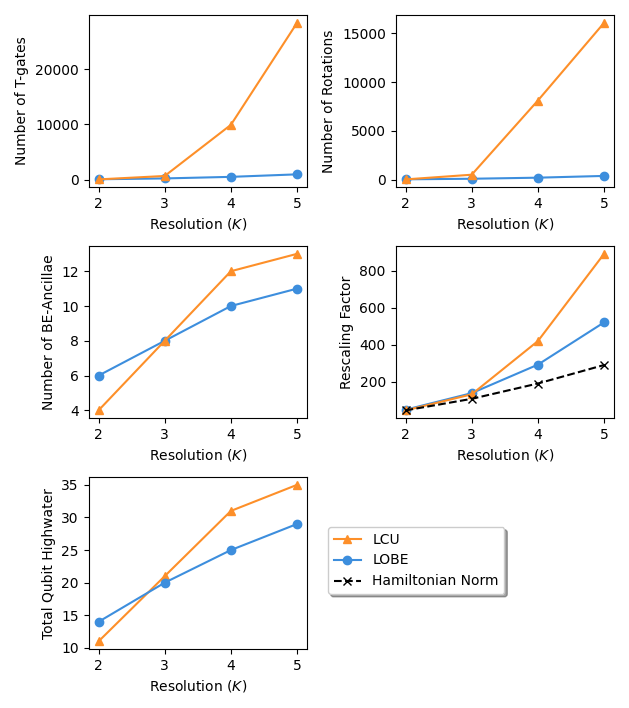
\includegraphics[width = 15cm]{figures/phi4_resolutions.png}
    \caption{}
    \label{}
\end{figure}

\begin{figure}[h]
    \centering
    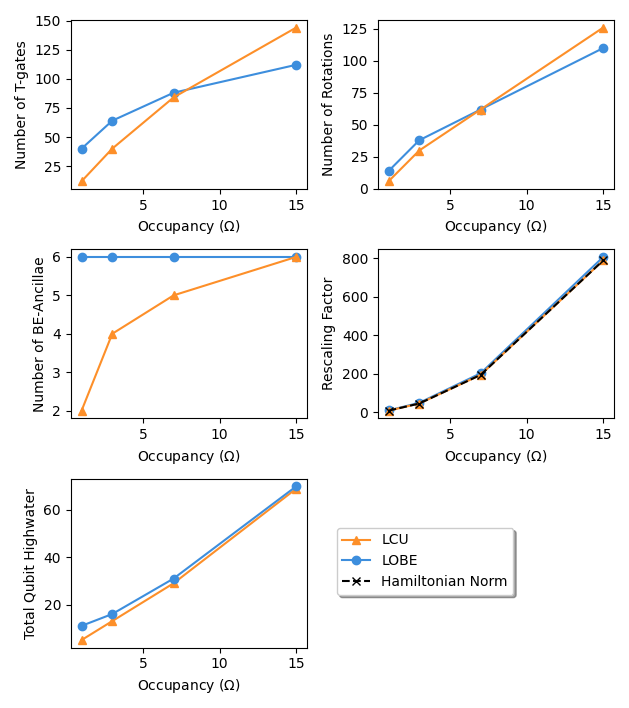
\includegraphics[width = 15cm]{figures/phi4_occupancies.png}
    \caption{}
    \label{}
\end{figure}